\begin{figure*}[t]
	\ifdefined\variantname\centering{\bfseries\variantname\par}\medskip\fi  % page label for main.tex only
	\centering
	\begin{subfigure}[b]{0.32\textwidth}
		\centering
		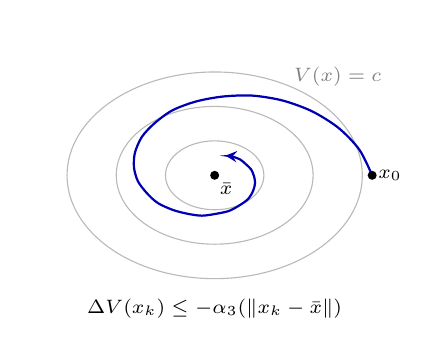
\begin{tikzpicture}[scale=1.25, >=stealth]
			\foreach \r in {0.5,1.0,1.5} {\draw[gray!55, thin] (0,0) ellipse ({\r} and {0.7*\r});}
			\node[gray, font=\scriptsize] at (1.25,1.0) {$V(x)=c$};
			\draw[thick, blue!70!black, ->] plot[smooth] coordinates {(1.60,0.00) (1.47,0.26) (1.26,0.48) (0.99,0.65) (0.69,0.76) (0.38,0.81) (0.08,0.80) (-0.19,0.75) (-0.43,0.66) (-0.61,0.53) (-0.74,0.39) (-0.81,0.23) (-0.82,0.08) (-0.78,-0.06) (-0.69,-0.18) (-0.58,-0.28) (-0.43,-0.35) (-0.28,-0.39) (-0.13,-0.41) (0.02,-0.39) (0.15,-0.36) (0.26,-0.30) (0.34,-0.24) (0.39,-0.16) (0.41,-0.08) (0.40,-0.01) (0.37,0.06) (0.32,0.11) (0.26,0.16) (0.18,0.19) (0.11,0.20)};
			\fill (0,0) circle (1.3pt);
			\node[font=\scriptsize, below right, inner sep=1pt] at (0.02,-0.05) {$\bar x$};
			\fill (1.6,0) circle (1.3pt);
			\node[font=\scriptsize, right, inner sep=2pt] at (1.6,0) {$x_0$};
			\node[font=\scriptsize] at (0,-1.35) {$\Delta V(x_k) \le -\alpha_3(\|x_k-\bar x\|)$};
			\path (-1.9,-1.5) rectangle (1.9,1.5);
		\end{tikzpicture}
		\caption{\edits{Nominal stability}}
		\label{fig:ss_nominal}
	\end{subfigure}%
	\begin{subfigure}[b]{0.32\textwidth}
		\centering
		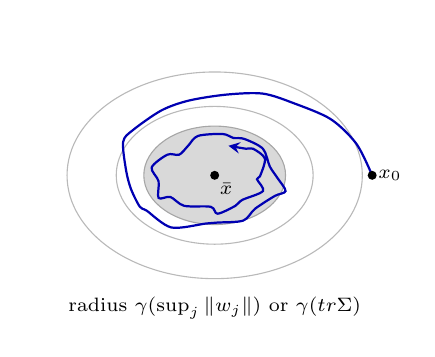
\begin{tikzpicture}[scale=1.25, >=stealth]
			\foreach \r in {1.0,1.5} {\draw[gray!55, thin] (0,0) ellipse ({\r} and {0.7*\r});}
			\fill[gray!30] (0,0) ellipse (0.72 and 0.5);
			\draw[gray!70, thin] (0,0) ellipse (0.72 and 0.5);
			\draw[thick, blue!70!black, ->] plot[smooth] coordinates {(1.60,0.00) (1.44,0.32) (1.18,0.57) (0.81,0.73) (0.49,0.83) (0.12,0.82) (-0.26,0.76) (-0.54,0.66) (-0.83,0.46) (-0.93,0.34) (-0.90,0.05) (-0.85,-0.14) (-0.76,-0.32) (-0.69,-0.36) (-0.44,-0.53) (-0.09,-0.49) (0.03,-0.48) (0.29,-0.46) (0.41,-0.34) (0.61,-0.21) (0.72,-0.16) (0.64,-0.03) (0.56,0.09) (0.49,0.27) (0.30,0.37) (0.19,0.38) (0.08,0.42) (-0.17,0.40) (-0.27,0.30) (-0.36,0.21) (-0.48,0.21) (-0.64,0.08) (-0.57,-0.06) (-0.57,-0.23) (-0.45,-0.22) (-0.31,-0.31) (-0.04,-0.32) (0.03,-0.39) (0.21,-0.31) (0.28,-0.25) (0.49,-0.16) (0.43,-0.04) (0.46,-0.01) (0.51,0.17) (0.39,0.27) (0.32,0.27) (0.14,0.30)};
			\fill (0,0) circle (1.3pt);
			\node[font=\scriptsize, below right, inner sep=1pt] at (0.02,-0.05) {$\bar x$};
			\fill (1.6,0) circle (1.3pt);
			\node[font=\scriptsize, right, inner sep=2pt] at (1.6,0) {$x_0$};
			\node[font=\scriptsize] at (0,-1.35) {radius $\gamma(\sup_j\|w_j\|)$ or $\gamma(\operatorname{tr}\Sigma)$};
			\path (-1.9,-1.5) rectangle (1.9,1.5);
		\end{tikzpicture}
		\caption{\edits{Robust and stochastic stability}}
		\label{fig:ss_robust}
	\end{subfigure}%
	\begin{subfigure}[b]{0.32\textwidth}
		\centering
		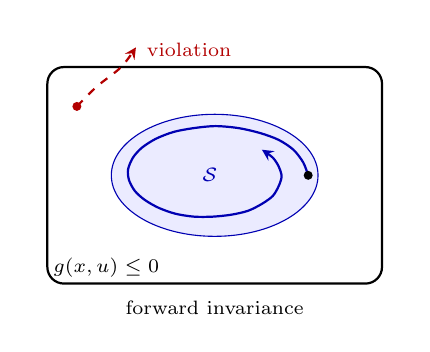
\begin{tikzpicture}[scale=1.25, >=stealth]
			\draw[thick, rounded corners=6pt] (-1.7,-1.1) rectangle (1.7,1.1);
			\node[font=\scriptsize, above right, inner sep=2pt] at (-1.7,-1.1) {$g(x,u)\le 0$};
			\fill[blue!8] (0,0) ellipse (1.05 and 0.62);
			\draw[blue!70!black, thin] (0,0) ellipse (1.05 and 0.62);
			\node[font=\scriptsize, blue!70!black] at (-0.05,0) {$\mathcal S$};
			\draw[thick, blue!70!black, ->] plot[smooth] coordinates {(0.95,0.00) (0.90,0.13) (0.80,0.26) (0.65,0.36) (0.46,0.43) (0.24,0.48) (0.01,0.50) (-0.21,0.48) (-0.42,0.44) (-0.60,0.37) (-0.74,0.28) (-0.83,0.18) (-0.88,0.06) (-0.87,-0.05) (-0.81,-0.16) (-0.71,-0.25) (-0.57,-0.33) (-0.40,-0.39) (-0.21,-0.42) (-0.02,-0.42) (0.17,-0.40) (0.34,-0.36) (0.48,-0.29) (0.59,-0.21) (0.65,-0.11) (0.68,-0.01) (0.65,0.09) (0.59,0.18) (0.48,0.26)};
			\fill (0.95,0) circle (1.3pt);
			\fill[red!70!black] (-1.4,0.7) circle (1.3pt);
			\draw[thick, red!70!black, dashed, ->] plot[smooth] coordinates {(-1.4,0.7) (-1.2,0.9) (-0.95,1.1) (-0.8,1.3)};
			\node[font=\scriptsize, red!70!black, right, inner sep=2pt] at (-0.75,1.28) {violation};
			\node[font=\scriptsize] at (0,-1.35) {forward invariance};
			\path (-1.9,-1.5) rectangle (1.9,1.5);
		\end{tikzpicture}
		\caption{\edits{Invariance and safety}}
		\label{fig:ss_invariance}
	\end{subfigure}\\[0.8em]
	\begin{subfigure}[b]{0.32\textwidth}
		\centering
		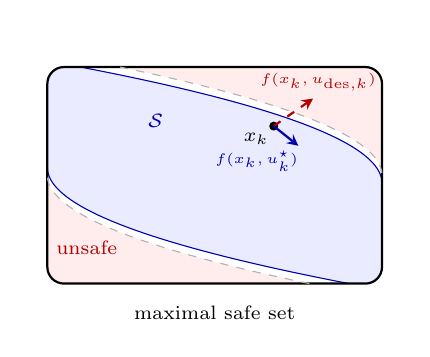
\begin{tikzpicture}[scale=1.25, >=stealth]
			% The red slivers along the right edge (moving right too fast) and the left edge (moving left too
			% fast) are the constraint-violating, unsafe states, as for a double integrator with a position
			% bound. The maximal safe set S is the largest invariant set within the constraints: its boundary
			% is the same parabola shifted along the box edge by \sfmargin, which leaves a white strip of about
			% \sfmargin between S and the unsafe states (closing only at the cusps on the left and right edges).
			\def\sfmargin{0.08}
			\begin{scope}
				\clip[rounded corners=6pt] (-1.7,-1.1) rectangle (1.7,1.1);
				\fill[red!7] (1.7,1.1) -- plot[variable=\t, domain=0:1.1, samples=30] ({1.7-2.2*(1.1-\t)*(1.1-\t)},{1.1-\t}) -- cycle;
				\fill[red!7] (-1.7,-1.1) -- plot[variable=\t, domain=0:1.1, samples=30] ({-1.7+2.2*(1.1-\t)*(1.1-\t)},{-1.1+\t}) -- cycle;
				\fill[blue!8] (-1.7,1.1) -- plot[variable=\t, domain=0:1.1+\sfmargin, samples=40] ({1.7-2.2*(1.1+\sfmargin-\t)*(1.1+\sfmargin-\t)},{1.1-\t}) -- (1.7,-1.1) -- plot[variable=\t, domain=0:1.1+\sfmargin, samples=40] ({-1.7+2.2*(1.1+\sfmargin-\t)*(1.1+\sfmargin-\t)},{-1.1+\t}) -- cycle;
				\draw[blue!70!black, thin] plot[variable=\t, domain=0:1.1+\sfmargin, samples=40] ({1.7-2.2*(1.1+\sfmargin-\t)*(1.1+\sfmargin-\t)},{1.1-\t});
				\draw[blue!70!black, thin] plot[variable=\t, domain=0:1.1+\sfmargin, samples=40] ({-1.7+2.2*(1.1+\sfmargin-\t)*(1.1+\sfmargin-\t)},{-1.1+\t});
			\end{scope}
			\draw[thick, rounded corners=6pt] (-1.7,-1.1) rectangle (1.7,1.1);
			% the edge of the unsafe region, dashed
			\draw[gray!60, dashed, thin] plot[variable=\t, domain=0:1.1, samples=30] ({1.7-2.2*(1.1-\t)*(1.1-\t)},{1.1-\t});
			\draw[gray!60, dashed, thin] plot[variable=\t, domain=0:1.1, samples=30] ({-1.7+2.2*(1.1-\t)*(1.1-\t)},{-1.1+\t});
			\node[font=\scriptsize, blue!70!black] at (-0.6,0.55) {$\mathcal S$};
			\node[font=\scriptsize, red!70!black] at (-1.3,-0.74) {unsafe};
			\node[font=\scriptsize] at (0,-1.4) {maximal safe set};
			\fill (0.6,0.5) circle (1.3pt);
			\node[font=\scriptsize, below left, inner sep=1pt] at (0.58,0.46) {$x_k$};
			\draw[thick, red!70!black, dashed, ->] (0.6,0.5) -- (1.0,0.78);
			\node[font=\tiny, red!70!black, above, inner sep=1pt] at (1.05,0.82) {$f(x_k,u_{\mathrm{des},k})$};
			\draw[thick, blue!70!black, ->] (0.6,0.5) -- (0.85,0.3);
			\node[font=\tiny, blue!70!black, below left, inner sep=1pt] at (0.88,0.28) {$f(x_k,u_k^\star)$};
			\path (-1.9,-1.5) rectangle (1.9,1.5);
		\end{tikzpicture}
		\caption{\edits{Hamilton-Jacobi reachability}}
		\label{fig:ss_hj}
	\end{subfigure}%
	\begin{subfigure}[b]{0.32\textwidth}
		\centering
		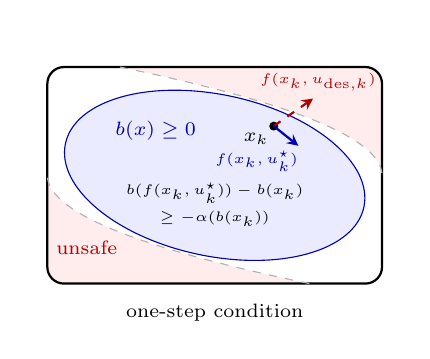
\begin{tikzpicture}[scale=1.25, >=stealth]
			% the unsafe states of (d), shaded as in (d)
			\begin{scope}
				\clip[rounded corners=6pt] (-1.7,-1.1) rectangle (1.7,1.1);
				\fill[red!7] (1.7,1.1) -- plot[variable=\t, domain=0:1.1, samples=30] ({1.7-2.2*(1.1-\t)*(1.1-\t)},{1.1-\t}) -- cycle;
				\fill[red!7] (-1.7,-1.1) -- plot[variable=\t, domain=0:1.1, samples=30] ({-1.7+2.2*(1.1-\t)*(1.1-\t)},{-1.1+\t}) -- cycle;
			\end{scope}
			\draw[thick, rounded corners=6pt] (-1.7,-1.1) rectangle (1.7,1.1);
			% the edge of the unsafe region, dashed
			\draw[gray!60, dashed, thin] plot[variable=\t, domain=0:1.1, samples=30] ({1.7-2.2*(1.1-\t)*(1.1-\t)},{1.1-\t});
			\draw[gray!60, dashed, thin] plot[variable=\t, domain=0:1.1, samples=30] ({-1.7+2.2*(1.1-\t)*(1.1-\t)},{-1.1+\t});
			\node[font=\scriptsize, red!70!black] at (-1.3,-0.74) {unsafe};
			\fill[blue!8, rotate=-12] (0,0) ellipse (1.55 and 0.82);
			\draw[blue!70!black, thin, rotate=-12] (0,0) ellipse (1.55 and 0.82);
			\node[font=\scriptsize, blue!70!black] at (-0.6,0.45) {$b(x)\ge0$};
			\node[font=\tiny, align=center] at (0.0,-0.3) {$b(f(x_k,u_k^\star)) - b(x_k)$\\[2pt]$\ge -\alpha(b(x_k))$};
			\node[font=\scriptsize] at (0,-1.4) {one-step condition};
			\fill (0.6,0.5) circle (1.3pt);
			\node[font=\scriptsize, below left, inner sep=1pt] at (0.58,0.46) {$x_k$};
			\draw[thick, red!70!black, dashed, ->] (0.6,0.5) -- (1.0,0.78);
			\node[font=\tiny, red!70!black, above, inner sep=1pt] at (1.05,0.82) {$f(x_k,u_{\mathrm{des},k})$};
			\draw[thick, blue!70!black, ->] (0.6,0.5) -- (0.85,0.3);
			\node[font=\tiny, blue!70!black, below left, inner sep=1pt] at (0.88,0.28) {$f(x_k,u_k^\star)$};
			\path (-1.9,-1.5) rectangle (1.9,1.5);
		\end{tikzpicture}
		\caption{\edits{Control barrier function}}
		\label{fig:ss_cbf}
	\end{subfigure}%
	\begin{subfigure}[b]{0.32\textwidth}
		\centering
		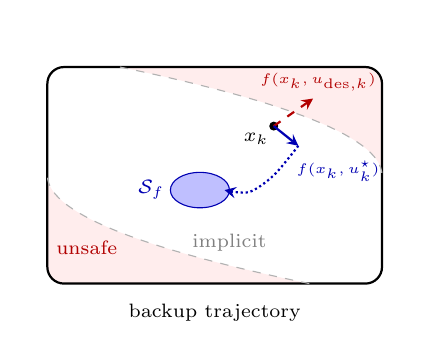
\begin{tikzpicture}[scale=1.25, >=stealth]
			% the unsafe states of (d), shaded as in (d)
			\begin{scope}
				\clip[rounded corners=6pt] (-1.7,-1.1) rectangle (1.7,1.1);
				\fill[red!7] (1.7,1.1) -- plot[variable=\t, domain=0:1.1, samples=30] ({1.7-2.2*(1.1-\t)*(1.1-\t)},{1.1-\t}) -- cycle;
				\fill[red!7] (-1.7,-1.1) -- plot[variable=\t, domain=0:1.1, samples=30] ({-1.7+2.2*(1.1-\t)*(1.1-\t)},{-1.1+\t}) -- cycle;
			\end{scope}
			\draw[thick, rounded corners=6pt] (-1.7,-1.1) rectangle (1.7,1.1);
			% the safe set is never computed
			% the edge of the unsafe region, dashed
			\draw[gray!60, dashed, thin] plot[variable=\t, domain=0:1.1, samples=30] ({1.7-2.2*(1.1-\t)*(1.1-\t)},{1.1-\t});
			\draw[gray!60, dashed, thin] plot[variable=\t, domain=0:1.1, samples=30] ({-1.7+2.2*(1.1-\t)*(1.1-\t)},{-1.1+\t});
			\node[font=\scriptsize, red!70!black] at (-1.3,-0.74) {unsafe};
			\node[font=\scriptsize, gray] at (0.15,-0.68) {implicit};
			\fill[blue!25] (-0.15,-0.15) ellipse (0.3 and 0.18);
			\draw[blue!70!black, thin] (-0.15,-0.15) ellipse (0.3 and 0.18);
			\node[font=\scriptsize, blue!70!black, left, inner sep=2pt] at (-0.45,-0.15) {$\mathcal S_f$};
			\node[font=\scriptsize] at (0,-1.4) {backup trajectory};
			\fill (0.6,0.5) circle (1.3pt);
			\node[font=\scriptsize, below left, inner sep=1pt] at (0.58,0.46) {$x_k$};
			\draw[thick, red!70!black, dashed, ->] (0.6,0.5) -- (1.0,0.78);
			\node[font=\tiny, red!70!black, above, inner sep=1pt] at (1.05,0.82) {$f(x_k,u_{\mathrm{des},k})$};
			\draw[thick, blue!70!black, ->] (0.6,0.5) -- (0.85,0.3);
			\node[font=\tiny, blue!70!black, right, inner sep=1pt] at (0.8,0.04) {$f(x_k,u_k^\star)$};
			\draw[blue!70!black, densely dotted, thick, ->] plot[smooth] coordinates {(0.85,0.3) (0.6,0.0) (0.35,-0.17) (0.1,-0.15)};
			\path (-1.9,-1.5) rectangle (1.9,1.5);
		\end{tikzpicture}
		\caption{\edits{Predictive safety filter}}
		\label{fig:ss_psf}
	\end{subfigure}
	\caption{\edits{Illustration of the stability and safety notions of this section. (a) Nominal stability: a Lyapunov function $V$ decreases along closed-loop trajectories (level sets in gray) and the state converges to the equilibrium $\bar x$. (b) Robust and stochastic stability: under disturbances $w$, the state converges to a neighbourhood of $\bar x$ (shaded), whose size depends on the disturbance bound or the noise covariance. (c) Safety: constraint satisfaction at one time instant does not imply safety (red dashed); safety is guaranteed by an invariant set $\mathcal S$ contained in the constraints. (d)--(f) Safety filters: the desired input $u_{\mathrm{des},k}$ would leave the safe set and is modified to $u_k^\star$; the unsafe states are shaded red (edge dashed). HJ reachability computes the maximal safe set $\mathcal S$ offline, the largest invariant set within the constraints. A CBF certifies invariance of $\{b(x)\ge0\}$ by the one-step condition on $b(x_{k+1})$. A PSF does not compute the safe set but certifies safety by a backup trajectory (dotted) into a smaller terminal set $\mathcal S_f$. }}
	\label{fig:stability_safety}
\end{figure*}
